%!TEX program = lualatex
\documentclass[11pt]{article}
\usepackage[a4paper, margin=1in, includehead]{geometry}
\geometry{a4paper} 
\usepackage[table, svgnames, dvipsnames]{xcolor}
\usepackage{makecell, cellspace, caption}
\usepackage[utf8]{inputenc}
\usepackage{textcomp}
\usepackage[most]{tcolorbox}
\usepackage{enumitem}
\usepackage{multicol}
\usepackage{graphicx} 
\usepackage{titling}
\usepackage{fancyhdr}
\usepackage{tabularray}
\pagestyle{fancy}
\fancyhf{}
\fancyhfoffset[L]{1cm} % left extra length
\fancyhfoffset[R]{1cm} % right extra length
\rhead{\textbf{\textit{Page-\thepage}}}
\lhead{\textbf{\textit{Software Requirements Specification for PedalPal}}}
\cfoot{}
\usepackage{amsmath,amssymb}  
\usepackage{bm}  
\usepackage[pdftex,bookmarks,colorlinks,breaklinks]{hyperref}  
\hypersetup{linkcolor=black,citecolor=black,filecolor=black,urlcolor=blue} % black links, for printed output
\usepackage{memhfixc} 
\usepackage{pdfsync}  
\usepackage{fancyhdr}
\usepackage{lmodern}
\usepackage{wrapfig}
\usepackage[page,toc,titletoc,title]{appendix}

\usepackage{fontspec}
\setmainfont{Arial}

\pagestyle{fancy}

\usepackage{titlesec}
\begin{document}
\begin{titlingpage}
\begin{flushright}
    \rule{16cm}{5pt}\vskip1cm
    \textbf{{\fontsize{30}{36}\selectfont Design Document}\\\vspace{1cm}\huge{for}\\\vspace{1cm}\Huge{PedalPal}\\ \vspace{1.5cm}\LARGE{Version 1.0}\\\vspace{1cm}\LARGE{Prepared by}}
\end{flushright}
\vspace{1.0cm}
\large{\begin{tabular*}{\columnwidth}{@{\extracolsep{\stretch{1}}}*{3}{c}@{}}
    \Large{\textbf{Group \# 4}} & & \Large{\textbf{Group Name: Bit Brewers}} \\
    \\
    \textbf{Raghav Manglik} & \textbf{220854} & \href{mailto:raghavkmanglik@gmail.com}{raghavkmanglik@gmail.com} \\
    \textbf{Amogh Bhagwat} & \textbf{220288} & \href{mailto:amogh.2004b@gmail.com}{amogh.2004b@gmail.com} \\
    \textbf{Srishti Chandra} & \textbf{221088} & \href{mailto:chandra.srishti2403@gmail.com}{chandra.srishti2403@gmail.com} \\
    \textbf{Wadkar Srujan Nitin} & \textbf{221212} & \href{mailto:srujanwadkar@gmail.com}{srujanwadkar@gmail.com} \\
    \textbf{Anaswar K B} & \textbf{220138} & \href{mailto:anaswarkb013@gmail.com}{anaswarkb013@gmail.com} \\
    \textbf{Khushi Gupta} & \textbf{220531} & \href{mailto:khushi07g@gmail.com}{khushi07g@gmail.com} \\
    \textbf{Ananya Singh Baghel} & \textbf{220136} & \href{mailto:ananyabaghel2004@gmail.com}{ananyabaghel2004@gmail.com} \\
    \textbf{Pathe Nevish Ashok} & \textbf{220757} & \href{mailto:nevu.pathe1234@gmail.com}{nevu.pathe1234@gmail.com} \\
    \textbf{Debraj Karmakar} & \textbf{220329} & \href{mailto:debraj2003jsr@gmail.com}{debraj2003jsr@gmail.com} \\
    \textbf{Kaneez Fatima} & \textbf{220496} & \href{mailto:kaneezfatimamehdi7@gmail.com}{kaneezfatimamehdi7@gmail.com} \\
    
\end{tabular*}}

\vspace{1.5cm}
\begin{center}
\large{
\begin{tabular}{l l}
    \textbf{Course:} & \textbf{CS253} \\
    \textbf{Mentor TA:} & \textbf{Mr. Bharat} \\
    \textbf{Instructor:} & \textbf{Prof. Indranil Saha} \\
    \textbf{Date:} & \textbf{February 9, 2024}
\end{tabular}
}
\end{center}
\end{titlingpage}

\titleformat{name=\section}[block]
  {\sffamily\LARGE}
  {}
  {0pt}
  {\colorsectionx}
\titlespacing*{\section}{0pt}{\baselineskip}{\baselineskip}
\newcommand{\colorsectionx}[1]{\colorbox{gray!120}{\parbox{\dimexpr\textwidth-2\fboxsep}{\color{white} \centering \huge{\textbf{Contents}}}}}

\tableofcontents

\newpage
\titleformat{name=\section}[block]
  {\sffamily\LARGE}
  {}
  {0pt}
  {\colorsection}
\titlespacing*{\section}{0pt}{\baselineskip}{\baselineskip}

\newcommand{\colorsection}[1]{\colorbox{gray!120}{\parbox{\dimexpr\textwidth-2\fboxsep}{\color{white}\huge{\textbf\thesection. }\ #1}}}

\section{\centering{\textbf{Revisions}}}
\begin{center}
\begin{tabular}{|c|c|c|c|}
    \hline
    \rowcolor{Gainsboro!60}
    \textbf{Version} & \textbf{Primary Author(s)} & \textbf{Description of Version} & \textbf{Date Completed} \\
    \hline
    \makecell{v1.0} & \makecell{Raghav Manglik \\ Amogh Bhagwat \\ Srishti Chandra \\ Wadkar Srujan Nitin \\ Pathe Nevish Ashok \\ Debraj Kamakar \\ Khushi Gupta \\ Ananya Baghel \\ Anaswar K B \\ Kaneez Fatima \\} & \makecell{First version of the \\Software Design Document} & \makecell{09/02/23} \\
    \hline
\end{tabular}
\end{center}

\newpage
\section{\centering{\textbf{Context Design}}}
\subsection{Context Model}
The context model of PedalPal is shown in the diagram. The context model shows the various entities that interact with the system, and the relationships between them. The entities are the user, the admin, the database, the payment gateway, the map, and the cycle lock. The user interacts with the system through the mobile app, while the admin interacts with the system through the web app. The database stores all the data of the system, while the payment gateway is used for the payment functionality. The map is used for the map functionality, and the microcontroller is used for the cycle lock functionality. The mail server is used to send password reset mails to the user.
\begin{center}
  \includegraphics[scale=0.1]{state-diagram-images/context-model.jpg}
\end{center}

\subsection{Human Interface Design}
\subsubsection{Login and Registration Pages}
\begin{figure}[h]
    \centering    
    \includegraphics[scale=0.35]{ui-images/Login.png}
    \hspace{30pt}
    \includegraphics[scale=0.35]{ui-images/Register.png}
    \hspace{30pt}
    \includegraphics[scale=0.35]{ui-images/ResetPassword.png}
\end{figure}
\begin{figure}[h]
    \centering    
    \includegraphics[scale=0.1]{ui-images/PhoneOTP.png}
    \hspace{20pt}
    \includegraphics[scale=0.35]{ui-images/EmailOTP.png}
    \hspace{20pt}
    \includegraphics[scale=0.1]{ui-images/AccountSuccess.png}
\end{figure}

\subsubsection{Booking a Ride}
\begin{center}
\begin{tabular}{ccc}
    \includegraphics[scale=0.35]{ui-images/Dashboard.png} &
    \includegraphics[scale=0.35]{ui-images/HubSelection.png} &
    \includegraphics[scale=0.1]{ui-images/BookRideSubscribed.png} \\
    \includegraphics[scale=0.35]{ui-images/QR.png} & \includegraphics[scale=0.1]{ui-images/ActiveRide.png} & \includegraphics[scale=0.1]{ui-images/RideOver.png}
\end{tabular}
\end{center}

\subsubsection{User Feedback}
\begin{center}
\begin{tabular}{ccc}
    \includegraphics[scale=0.1]{ui-images/CycleIssues.png} & \includegraphics[scale=0.1]{ui-images/IssueDescription.png} & \includegraphics[scale=0.1]{ui-images/FeedbackSubmission.png}
\end{tabular}
\end{center}

\subsubsection{Subscription Model}
\begin{center}
    \begin{tabular}{cc}
        \includegraphics[scale=0.1]{ui-images/BookRideUnsubscribed.png} & \includegraphics[scale=0.1]{ui-images/Advertisement.png}
    \end{tabular}
\end{center}

\subsubsection{Settings and Analytics View}
\begin{center}
\begin{tabular}{ccc}
    \includegraphics[scale=0.36]{ui-images/Navbar.png} & \includegraphics[scale=0.1]{ui-images/Wallet.png} & \includegraphics[scale=0.275]{ui-images/History.png}
\end{tabular}
\begin{tabular}{cc}
\includegraphics[scale=0.1]{ui-images/Settings.png} & \includegraphics[scale=0.1]{ui-images/Bookings.png}
\end{tabular}
\end{center}

\subsubsection{Admin Interface}
\begin{center}
    \begin{tabular}{c}
        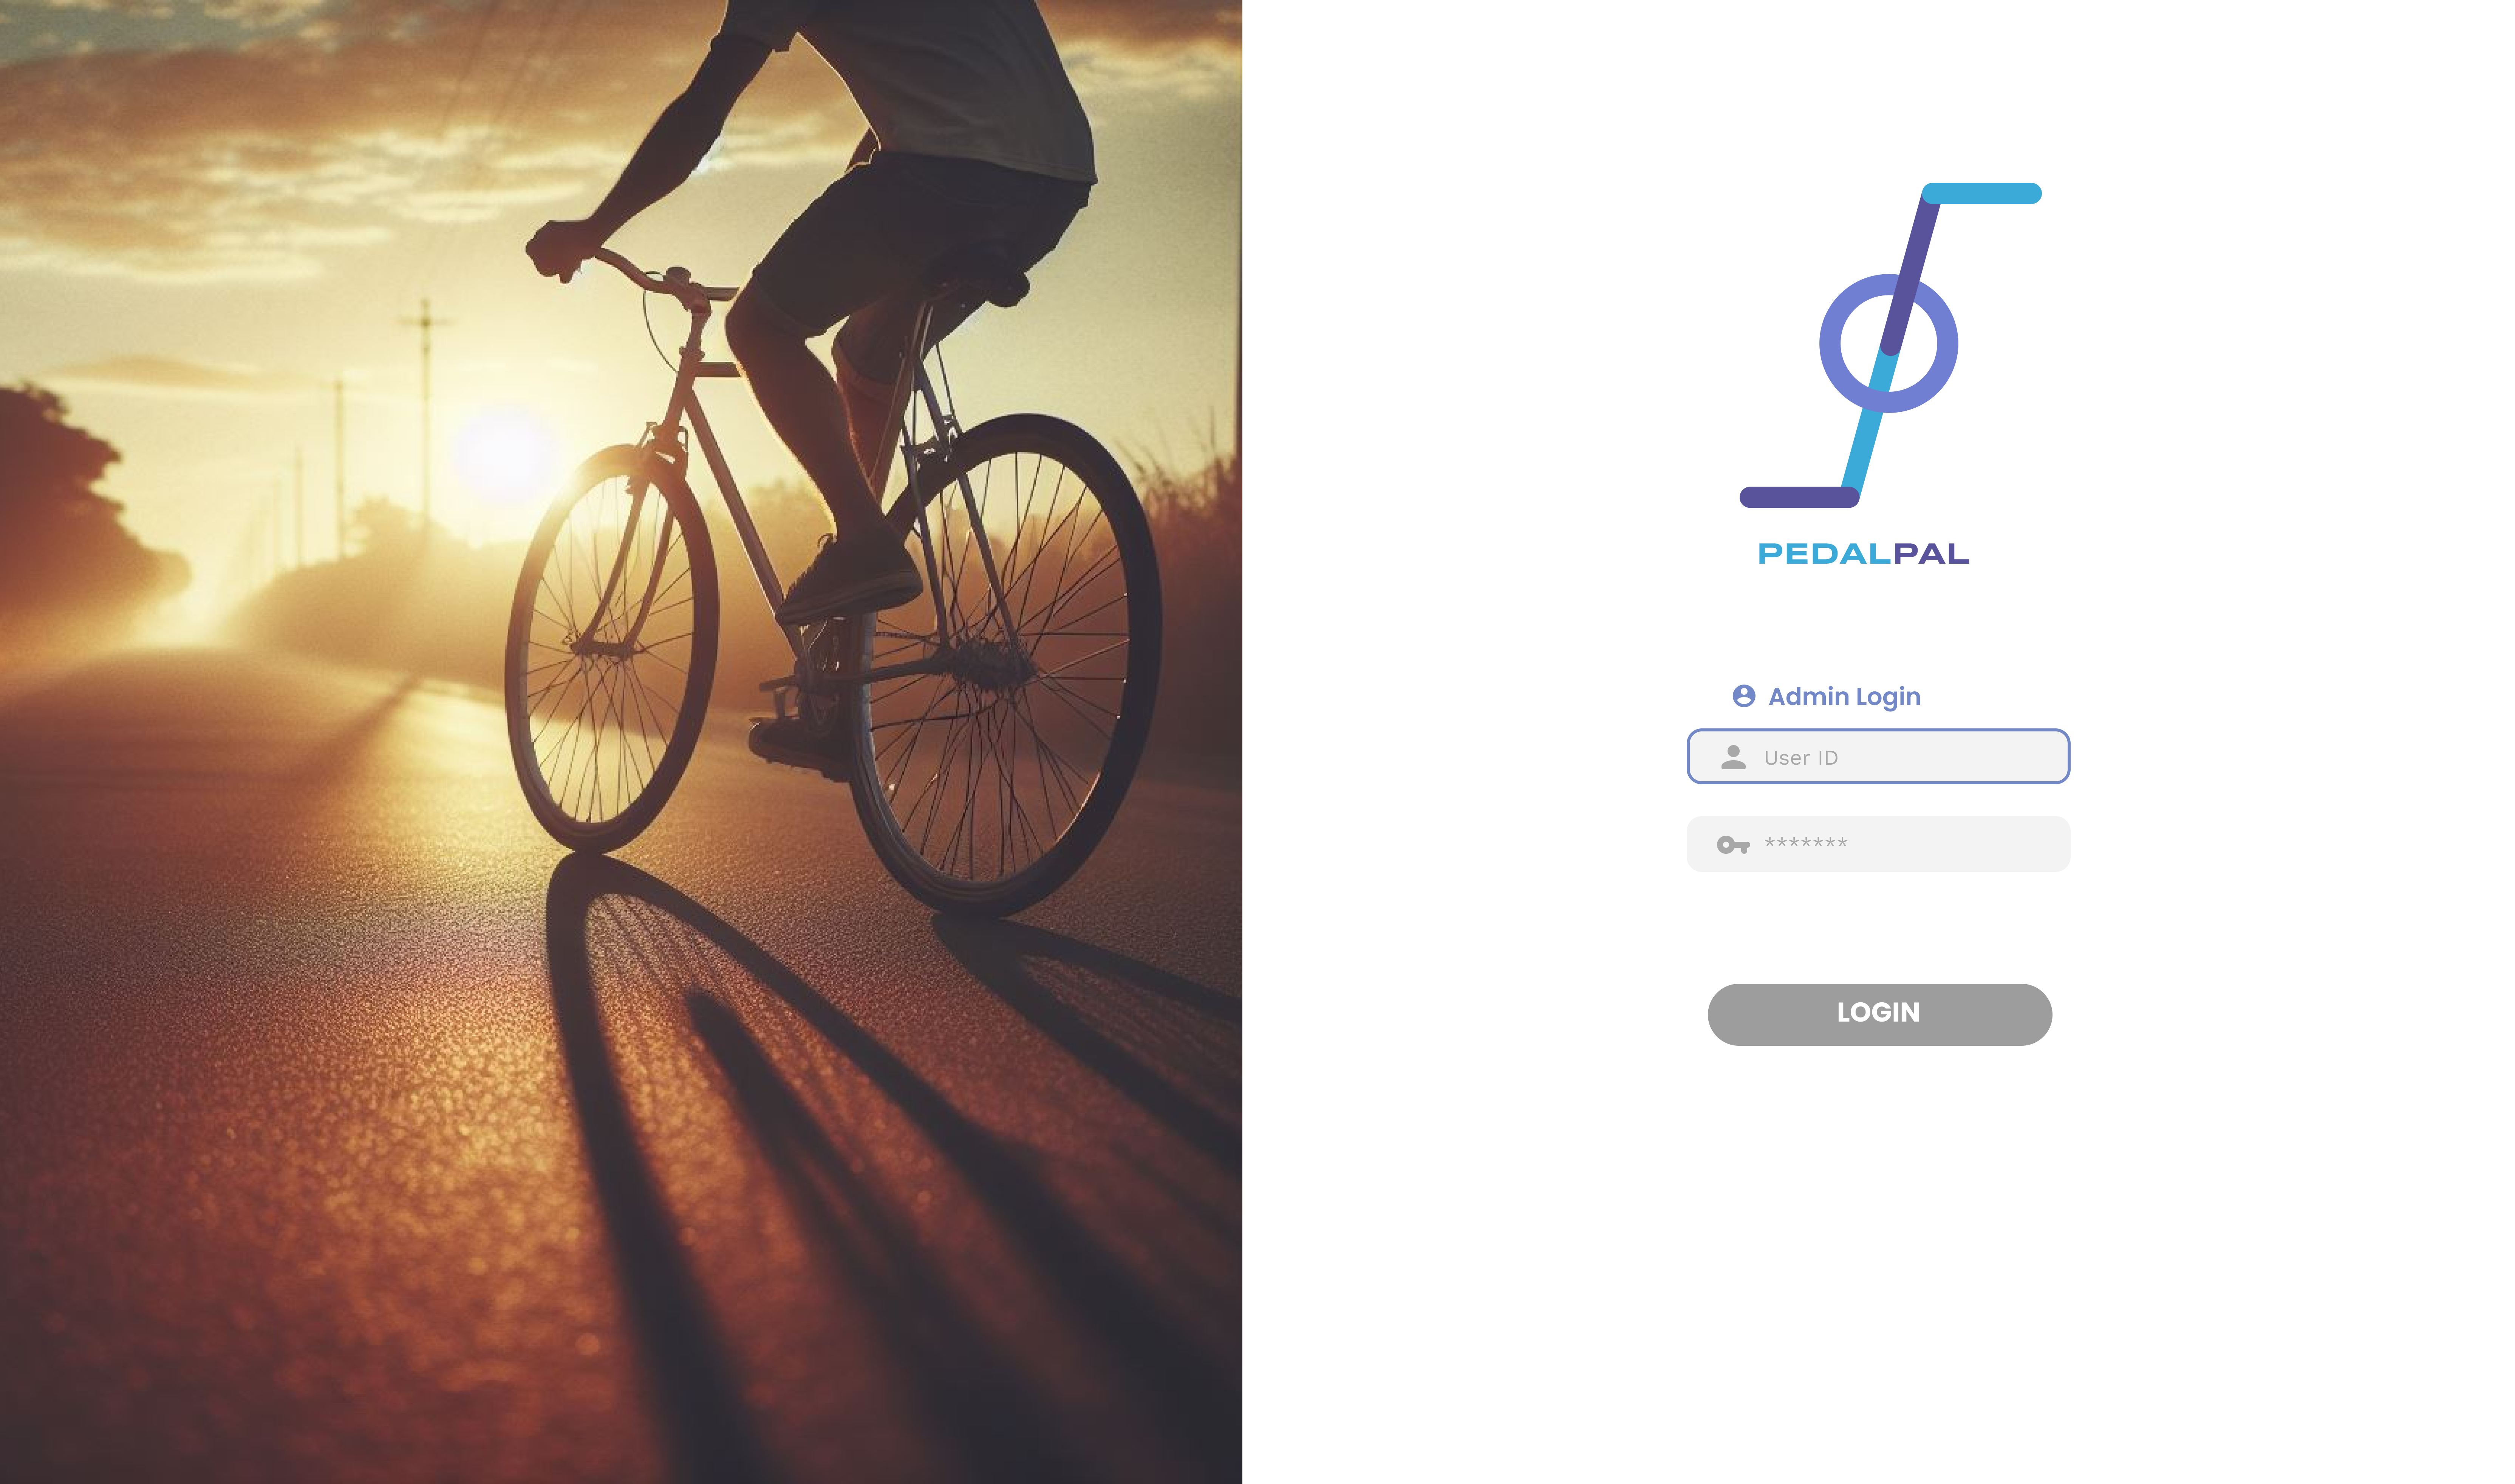
\includegraphics[scale=0.08]{ui-images/AdminLogin.png} \\
        \includegraphics[scale=0.08]{ui-images/AdminDashboard.png}
    \end{tabular}
\end{center}



\newpage
\section{\centering{\textbf{Architecture Design}}}
The overall architecture of our app follows the Model-View-Controller model. Given the complexity of the app, each functionality is sub-divided into smaller tasks, which are achieved by the Pipe-Filter architecture model.

The model-view-controller architecture is as follows:
\begin{itemize}
  \item \textbf{Model:} The model is the data layer of the app. It is the only layer that directly communicates with the database. It is responsible for the storage and retrieval of data from the database. We plan to use PostgreSQL as our database, while using Django as our backend framework to interact with the database.
  \item \textbf{View:} The view is the presentation layer of the app. It is responsible for the display of data to the user. It is also responsible for taking input from the user. The view for app users will be a mobile app, while the view for the admin will be a web app. The mobile app is planned to be built using Flutter, while the admin webpage is automatically generated by Django.
  \item \textbf{Controller:} The controller is the logic layer of the app. It is responsible for processing the data and deciding the flow of the app. The controller will be built using Django in the Python language. Google Maps API will be used for the map functionality, and RazorPay API will be used for the payment functionality. The hardware component of opening cycle lock will be handled by a microcontroller such as Arduino.
\end{itemize}
\begin{center}
  \includegraphics[scale=0.2]{architecture-images/overall.png}
\end{center}

\newpage
\section{\centering{\textbf{Object Oriented Design}}}
\subsection{Use Case Diagrams}
Overview of the use cases of PedalPal is as follows
\begin{center}
  \includegraphics[scale=0.75]{../srs/Overview.png}
    \includegraphics[scale=0.25]{../srs/usecase.png}
\end{center}
The various use cases are as follows
\subsubsection{Use Case 1 (U1) - Ability to Start Ride and End Ride}
\begin{center}
  \includegraphics[scale=0.5]{../srs/usecase-1.png}
\end{center}

\subsubsection{Use Case 2 (U2) - Ability to View Nearby Hubs on a Map}
\begin{center}
  \includegraphics[scale=0.5]{../srs/usecase-2.png}
\end{center}

\subsubsection{Use Case 3 (U3) - Ability to Create a new Account}
\begin{center}
  \includegraphics[scale=0.5]{../srs/usecase-3.png}
\end{center}

\subsubsection{Use Case 4 (U4) - Ability to View Analytics}
\begin{center}
  \includegraphics[scale=0.5]{../srs/usecase-4.png}
\end{center}

\subsubsection{Use Case 5 (U5) - Feedback Mechanism}
\begin{center}
  \includegraphics[scale=0.5]{../srs/usecase-5.png}
\end{center}

\subsubsection{Use Case 6 (U6) - Ability to Use and Recharge Wallet}
\begin{center}
  \includegraphics[scale=0.5]{../srs/usecase-6.png}
\end{center}

\subsection{Class Diagrams}
\begin{center}
  \includegraphics[scale=0.1]{class-diagram-images/overall.jpg}
\end{center}

\subsection{Sequence Diagrams}
\subsubsection{Login Sequence}
\begin{center}
  \includegraphics[scale=0.35]{sequence-diagram-images/login.png}
\end{center}

\subsubsection{Registration Sequence}
\begin{center}
  \includegraphics[scale=0.3]{sequence-diagram-images/register.png}
\end{center}

\subsubsection{Reset Password Sequence}
\begin{center}
  \includegraphics[scale=0.35]{sequence-diagram-images/reset_password.png}
\end{center}

\subsubsection{Fetch Cycle Hubs Sequence}
\begin{center}
  \includegraphics[scale=0.28]{sequence-diagram-images/fetch_hubs.png}
\end{center}

\subsubsection{Book Ride Sequence}
\begin{center}
  \includegraphics[scale=0.27]{sequence-diagram-images/book.png}
\end{center}

\subsubsection{Payment Sequence}
\begin{center}
  \includegraphics[scale=0.28]{sequence-diagram-images/payment.png}
\end{center}

\subsubsection{Feedback Sequence}
\begin{center}
  \includegraphics[scale=0.35]{sequence-diagram-images/feedback.png}
\end{center}

\subsubsection{View Analytics Sequence}
\begin{center}
  \includegraphics[scale=0.3]{sequence-diagram-images/analytics.png}
\end{center}

\subsubsection{Admin Sequence}
\begin{center}
  \includegraphics[scale=0.3]{sequence-diagram-images/admin.png}
\end{center}


\subsection{State Diagrams}
\subsubsection{Overall state diagram}
\begin{center}
  \includegraphics[scale=0.105]{state-diagram-images/overall.png}
\end{center}

The image describes the high-level state diagram of the application from a user perspective. The customer can either be a subscribed customer or an unsubscribed customer. The customer can book a ride, view ride history, view wallet, view settings, view booking history, and give feedback. The orange boxes show a query to the database and the red diamonds show a decision point.

\subsubsection{Ride Begin state diagram}
\begin{center}
  \includegraphics[scale=0.25]{state-diagram-images/ride_begin.jpg}
\end{center}

\subsubsection{Ride End state diagram}
\begin{center}
  \includegraphics[scale=0.2]{state-diagram-images/ride_end.jpg}
\end{center}

\newpage
\section{\centering{\textbf{Project Plan}}}
\subsection{Project Planning}
We are using Notion to track the progress and deadlines of the project. It also allows us to assign tasks to team members. The current Gantt chart looks like this:
\begin{center}
  \includegraphics[scale=0.1]{project-plan-images/notion.png}
\end{center}

\subsection{Code Collaboration}
We are using GitHub to collaborate on the code. An organization is created for the purposes of this project and all team members are added to this organization. Separate repositories are maintained for the backend and frontend of our app. 
\begin{center}
  \includegraphics[scale=0.3]{project-plan-images/github.png}
\end{center}

\subsection{Communication}
We are using Discord for communication. It allows us to create separate channels for different topics, and keep data organised. It also allows us to have voice calls and video calls, which is useful for team meetings.
\begin{center}
  \includegraphics[scale=0.3]{project-plan-images/communication.png}
\end{center}

% \newpage
% \section{\centering{\textbf{Other Details}}}

\newpage
\appendixpageoff
\begin{appendices}

\section{\centering{\textbf{Group Log}}}
\begin{tabular}{|p{1cm}|p{2cm}|p{2cm}|p{2cm}|p{6.75cm}|}
\hline
\makecell{\textbf{S.No}} & \makecell{\textbf{Date}} & \makecell{\textbf{Timings}} & \makecell{\textbf{Venue}} & \makecell{\textbf{Description}} \\
\hline
\makecell{1} & \makecell{31/01/2024} & \makecell{21:30\\ to \\23:00} & \makecell{Discord} & \makecell{Studied deliverables for the\\design document. \\ Divided work among teammates} \\
\hline
\makecell{2} & \makecell{03/02/2024} & \makecell{11:00\\to\\14:00} & \makecell{RM\\Building} & \makecell{Designed user interface\\Discussed project details\\like frameworks and other APIs} \\
\hline
\makecell{3} & \makecell{07/02/2024} & \makecell{21:30\\to\\22:00} & \makecell{Google\\Meet} & \makecell{Meet with TA to discuss details\\about the document.} \\
\hline
\makecell{4} & \makecell{08/02/2024} & \makecell{14:30\\to\\17:00} & \makecell{RM\\Building} & \makecell{Finalized all aspects of the \\ design document\\Decided future plans} \\
\hline
\end{tabular}
\end{appendices}
\end{document}
